% Begin the document and set up the style of the document
\documentclass[a4paper]{article}

% Install the required packages for the document 
\usepackage{envmath}
\usepackage{esvect}
\usepackage{graphicx}
\usepackage{gensymb}
\usepackage{tikz}
\usepackage[mathcal]{euscript}
\usepackage{geometry}
\usepackage{enumitem}
\usepackage{mathtools}
\usepackage{graphicx}
\usepackage{amsmath}
\usepackage{amscd}
\usepackage{amssymb}
\usepackage{amsfonts}
\usepackage{harpoon}
\usepackage{pgf}
\usepackage{tikz}
\usepackage{mathrsfs}
\usepackage{asyalign}
\usepackage{physics}
\usepackage{enumitem}
\usepackage{xhfill}
\usepackage{accents}
\usepackage{cite}
\usepackage{url}
\usepackage{csquotes}
\usepackage{wrapfig}
\usepackage{booktabs}
\usepackage{adjustbox}
\usepackage{caption}
\usepackage{minipage-marginpar}
\usepackage{calc}
\usepackage[tableposition=top]{caption}
\usepackage{ifthen}
\usepackage[utf8]{inputenc}
\usepackage{tikz-3dplot}
\usetikzlibrary{patterns}
\usetikzlibrary{arrows}

% Page and style settings
\parskip=8pt
\parindent=0pt
% Right margin
\textwidth=6.25in
% Left margin
\oddsidemargin=0pt
\evensidemargin=0pt
% Bottom margin
\textheight=10in
% Top margin
\topmargin=-0.75in
\baselineskip=11pt
% end of page and other style settings

\renewcommand{\familydefault}{\sfdefault}

\newcommand{\indep}{\mathrel{\text{\scalebox{1.07}{$\perp\mkern-10mu\perp$}}}}
\newcommand{\p}{\mathbb{P}}
\newcommand{\e}{\mathbb{E}}
\newcommand{\ds}{\displaystyle}
\newcommand{\code}{\texttt}

% Begin the text of the document
\begin{document}

\newlength{\strutheight}
\settoheight{\strutheight}{\strut}

% Begin the Title Page
\begin{titlepage}

\newcommand{\HRule}{\rule{\linewidth}{0.5mm}} % Defines a new command for the horizontal lines, change thickness here

\center % Center everything on the page
 
\textsc{\LARGE University of New South Wales}\\[1.5cm] % Name of your university/college
\textsc{\Large MATH 2901}\\[0.5cm] % Major heading such as course name
\textsc{\large Higher Theory of Statistics}\\[0.5cm] % Minor heading such as course title

\HRule \\[0.4cm]
{ \huge \bfseries Assignment 1}\\[0.4cm] % Title of your document
\HRule \\[1.5cm]


\begin{center} \large
Keegan Gyoery (z5197058), Edward McInnes (z5162873),\\ Alex Robinson (z5164884), Ruby Smith (z5113171) % Your name
\\
\end{center}


\vspace{4cm}

{\today}\\[3cm] % Date, change the \today to a set date if you want to be precise

\vfill % Fill the rest of the page with whitespace

\end{titlepage}

\pagenumbering{arabic}


\begin{enumerate}

	\item 
	\begin{enumerate}

		\item If event $\ds{A}$ is independent of itself, by the definition of independence, the following result holds.

		\begin{align*}
			\p(A \cap A) & = \p(A)\p(A) \hspace{5mm} \text{definition of independence} \\
			& = \big[\p(A) \big] ^2 \hspace{5mm} \text{as $\ds{\p(A \cap A) = \p(A)}$}\\
			\p(A) & = \big[\p(A) \big] ^2 \\
			\therefore \big[\p(A) \big] ^2 - \p(A) & = 0 \\
			\therefore \p(A)\big[\p(A) - 1 \big]  & = 0 \\
			\therefore \p(A) & = 0 \hspace{5mm} \text{OR} \\
			\p(A) & = 1 \\
		\end{align*}

		\item Suppose that event $\ds{A}$ has probability $\ds{\p(A) = 1}$, and the event $\ds{B}$ has some probability $\ds{\p(B)}$. Thus the following consequences arise.

		\begin{align*}
			\p(A \cap B) & = \p(B) \hspace{5mm} \text{as $B \subseteq A$}\\
			& = 1 \times \p(B) \\
			& = \p(A)\p(B) \\
			\therefore \p(A \cap B) & = \p(A)\p(B) \\
		\end{align*}

		Thus if event $\ds{A}$ has probability $\ds{\p(A) = 1}$, events $\ds{A}$ and $\ds{B}$ are independent.

		\bigbreak

		Suppose now that event $\ds{A}$ has probability $\ds{\p(A) = 0}$, and the event $\ds{B}$ has some probability $\ds{\p(B)}$.

		\begin{align*}
			\p(A \cap B) & = 0 \hspace{5mm} \text{as $A \subseteq B$}\\
			& = 0 \times \p(B) \\
			& = \p(A)\p(B) \\
			\therefore \p(A \cap B) & = \p(A)\p(B) \\
		\end{align*}

		Again, if event $\ds{A}$ has probability $\ds{\p(A) = 0}$, events $\ds{A}$ and $\ds{B}$ are independent.

	\end{enumerate}

	\bigbreak

	\item The following probability tree will be used to answer question 2. Furthermore, the notation $\ds{FC}$ will denote the Fair Coin.

	\begin{center}
		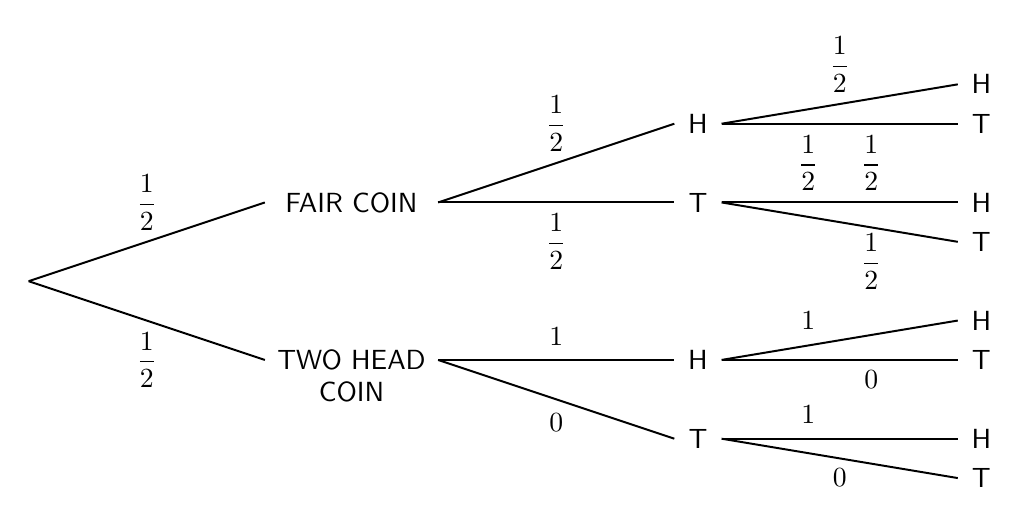
\begin{tikzpicture}

			\draw[line width = 0.25mm] (-4.5,0) -- (-1.5,1);
			\draw[line width = 0.25mm] (-4.5,0) -- (-1.5,-1);
			\node at (-0.4,1) {FAIR COIN};
			\node at (-0.4,-1) {TWO HEAD};
			\node at (-0.4,-1.4) {COIN};

			\draw[line width = 0.25mm] (0.7,1) -- (3.7,2);
			\draw[line width = 0.25mm] (0.7,-1) -- (3.7,-2);
			\draw[line width = 0.25mm] (0.7,1) -- (3.7,1);
			\draw[line width = 0.25mm] (0.7,-1) -- (3.7,-1);
			\node at (4,2) {H};
			\node at (4,1) {T};
			\node at (4,-1) {H};
			\node at (4,-2) {T};

			\draw[line width = 0.25mm] (4.3,2) -- (7.3,2.5);
			\draw[line width = 0.25mm] (4.3,2) -- (7.3,2);
			\draw[line width = 0.25mm] (4.3,1) -- (7.3,1);
			\draw[line width = 0.25mm] (4.3,1) -- (7.3,0.5);
			\draw[line width = 0.25mm] (4.3,-2) -- (7.3,-2.5);
			\draw[line width = 0.25mm] (4.3,-2) -- (7.3,-2);
			\draw[line width = 0.25mm] (4.3,-1) -- (7.3,-1);
			\draw[line width = 0.25mm] (4.3,-1) -- (7.3,-0.5);
			\node at (7.6,2) {T};
			\node at (7.6,2.5) {H};
			\node at (7.6,1) {H};
			\node at (7.6,0.5) {T};
			\node at (7.6,-2) {H};
			\node at (7.6,-2.5) {T};
			\node at (7.6,-1) {T};
			\node at (7.6,-0.5) {H};

			\node at (-3,1) {$\ds{\frac{1}{2}}$};
			\node at (-3,-1) {$\ds{\frac{1}{2}}$};
			\node at (2.2,2) {$\ds{\frac{1}{2}}$};
			\node at (2.2,0.5) {$\ds{\frac{1}{2}}$};
			\node at (2.2,-0.7) {$\ds{1}$};
			\node at (2.2,-1.8) {$\ds{0}$};
			\node at (5.8,2.75) {$\ds{\frac{1}{2}}$};
			\node at (5.4,1.5) {$\ds{\frac{1}{2}}$};
			\node at (6.2,1.5) {$\ds{\frac{1}{2}}$};
			\node at (5.4,-0.5) {$\ds{1}$};
			\node at (6.2,0.25) {$\ds{\frac{1}{2}}$};
			\node at (5.8,-2.5) {$\ds{0}$};
			\node at (5.4,-1.7) {$\ds{1}$};
			\node at (6.2,-1.25) {$\ds{0}$};

		\end{tikzpicture}
	\end{center}

	\pagebreak
		
	\begin{enumerate}

		\item 
		\begin{align*}
			\p(FC\:|\:H) & = \frac{\p(FC \cap H)}{\p(H)} \\
			& = \frac{\frac{1}{2}\times\frac{1}{2}}{\Big(\frac{1}{2}\times\frac{1}{2} \Big) + \Big(\frac{1}{2}\times1\Big)} \\
			& = \frac{\frac{1}{4}}{\frac{1}{4} + \frac{1}{2}} \\
			& = \frac{1}{3} \\
		\end{align*}

		Thus the probability of choosing the fair coin given that the coin shows heads after the first flip is $\ds{\frac{1}{3}}$

		\bigbreak

		\item
		\begin{align*}
			\p(FC\:|\:H,H) & = \frac{\p(FC \cap H,H)}{\p(H,H)} \\
			& = \frac{\frac{1}{2}\times\frac{1}{2}\times\frac{1}{2}}{\Big(\frac{1}{2}\times\frac{1}{2}\times\frac{1}{2}\Big) + \Big(\frac{1}{2}\times1\times1\Big)} \\
			& = \frac{\frac{1}{8}}{\frac{1}{8} + \frac{1}{2}} \\
			& = \frac{1}{5} \\
		\end{align*}

		Thus the probability of choosing the fair coin given that the coin shows heads after the first flip, and heads after the second flip, is $\ds{\frac{1}{5}}$

		\bigbreak
		
		\item
		\begin{align*}
			\p(FC\:|\:H,H,T) & = \frac{\p(FC \cap H,H,T)}{\p(H,H,T)} \\
			& = \frac{\frac{1}{2}\times\frac{1}{2}\times\frac{1}{2}\times\frac{1}{2}}{\Big(\frac{1}{2}\times\frac{1}{2}\times\frac{1}{2}\times\frac{1}{2}\Big) + \Big(\frac{1}{2}\times1\times1\times0\Big)} \\
			& = 1 \\
		\end{align*}

		Thus the probability of choosing the fair coin given that the coin shows heads after the first flip, heads after the second flip, and tails after the third flip, is $\ds{1}$

	\end{enumerate}

	\bigbreak

	\item For the following question, we will use the defined notation below.
	\begin{tabbing}
		$\ds{A}$ is the event tha\=t Bill hits the target \hspace{5mm}\=: $\ds{\p(A) = 0.7}$ \\
		$\ds{B}$ \"{} \>\"{} George hits the target \>: $\ds{\p(B) = 0.4}$ \\
		$\ds{C}$ \"{} \>\"{} the target is hit once \>: $\ds{\p(C) = 0.7\times0.6 + 0.3\times0.4 = 0.54}$ \\
		$\ds{D}$ \"{} \>\"{} the target is hit \>: $\ds{\p(D) = \p(C) + 0.7\times0.4 = 0.82}$ \\
	\end{tabbing}

	\pagebreak

	\begin{enumerate}

		\item 
		\begin{align*}
			\p(B|C) & = \frac{\p(B \cap C)}{\p(C)} \hspace{5mm} \text{[conditional probability]} \\
			& = \frac{0.3\times0.4}{0.54} \\
			& = \frac{2}{9} \\
		\end{align*}

		\item 
		\begin{align*}
			\p(B|D) & = \frac{\p(B \cap D)}{\p(D)} \hspace{5mm} \text{[conditional probability]} \\
			& = \frac{(0.3\times0.4) + (0.7\times0.4)}{0.82} \\
			& = \frac{20}{41} \\
		\end{align*}

	\end{enumerate}

	\bigbreak

	\item We want $\ds{\p(B|A) + \p(B|A^{c}) = 1}$ and $\ds{\p(B|A) + \p(B^{c}|A^{c}) = 1}$. Therefore, we need $\ds{\p(B|A^{c}) = \p(B|A^{c}) = \frac{1}{2}}$

	\begin{center}
		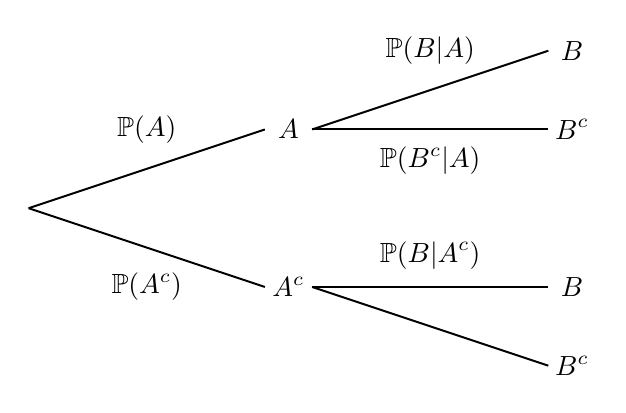
\begin{tikzpicture}

			\draw[line width = 0.25mm] (-4.5,0) -- (-1.5,1);
			\draw[line width = 0.25mm] (-4.5,0) -- (-1.5,-1);
			\node at (-1.2,1) {$\ds{A}$};
			\node at (-1.2,-1) {$\ds{A^{c}}$};

			\draw[line width = 0.25mm] (-0.9,1) -- (2.1,2);
			\draw[line width = 0.25mm] (-0.9,-1) -- (2.1,-2);
			\draw[line width = 0.25mm] (-0.9,1) -- (2.1,1);
			\draw[line width = 0.25mm] (-0.9,-1) -- (2.1,-1);
			\node at (2.4,2) {$\ds{B}$};
			\node at (2.4,1) {$\ds{B^{c}}$};
			\node at (2.4,-1) {$\ds{B}$};
			\node at (2.4,-2) {$\ds{B^{c}}$};

			\node at (-3,1) {$\ds{\p(A)}$};
			\node at (-3,-1) {$\ds{\p(A^{c})}$};
			\node at (0.6,2) {$\ds{\p(B|A)}$};
			\node at (0.6,0.6) {$\ds{\p(B^{c}|A)}$};
			\node at (0.6,-0.6) {$\ds{\p(B|A^{c})}$};

		\end{tikzpicture}
	\end{center}

	Let the event be the tossing of consecutive coins. Let $\ds{A}$ be heads and therefore $\ds{A^{c}}$ is tails. Let $\ds{B}$ be heads and therefore $\ds{B^{c}}$ is tails.

	\begin{align*}
		\p(B|A) & = \p(\text{Heads}|\text{Heads}) \\
		& = \frac{\p(\text{Heads} \cap \text{Heads})}{\p(\text{Heads})} \\
		& = \frac{\frac{1}{2}\times\frac{1}{2}}{\frac{1}{2}} \\
		& = \frac{1}{2} \\
		\text{Similarly, } \p(B|A^{c}) & = \p(B^{c}|A^{c}) \\
		& = \frac{1}{2} \\
	\end{align*}

	Therefore the final results are apparent.

	\begin{align*}
		\p(B|A) + \p(B|A^{c}) & = \frac{1}{2} + \frac{1}{2} = 1 \\
		\p(B|A) + \p(B^{c}|A^{c}) & = \frac{1}{2} + \frac{1}{2} = 1 \\
	\end{align*}

	\pagebreak

	\item 
	\begin{enumerate}

		\item 

		\begin{align*}
			F_X(x) & = \int_{-\infty}^x f_X(t) dt \\
			& = \int_{-\infty}^x \frac{2}{t^2} dt \\
			& = \bigg[\frac{-2}{t} \bigg]_{-\infty}^x \\
			& = \frac{-2}{x} \\
		\end{align*}

		\item 

		\begin{align*}
			\e(X) & = \int_1^2 xf_X(x) dx \\
			& = 2 \int_1^2 \frac{1}{x} dx \\
			& = 2 \ln{x} \hspace{0.75mm} \Big|_1^2 \\
			& = 2 [\ln{2} - \ln{1}] \\
			& = 2\ln{2} \\
		\end{align*}

		Let $\ds{M}$ be the location of the median.

		\begin{align*}
			F_X(x) & = \frac{1}{2} \\
			\therefore \frac{1}{2} & = \int_1^M f_X(x) dx \\
			& = 2 \int_1^M \frac{1}{x^2} dx \\
			& = 2 \bigg[\frac{-1}{x} \bigg]_1^M \\
			& = 2 \bigg[\frac{-1}{M} + 1 \bigg] \\
			& = \frac{-2}{M} + 2 \\
			\therefore \frac{2}{M} & = \frac{3}{2} \\
			\therefore M & = \frac{4}{3} \\
		\end{align*}


	\end{enumerate}

	\bigbreak

	\item If $\ds{X \sim \text{Bin}(n,p) \implies \p(X=x) = \binom{n}{k} p^{x}(1-p)^{n-x}}$. Furthermore,
	\begin{align*}
		\p(X= \text{even}) & = \p(X=0) + \p(X=2) + \dots + \p(X=k) \hspace{5mm} \text{where $\ds{k =}$}
		\begin{cases}
			n & \text{if $\ds{n}$ is even} \\
			n - 1 & \text{if $\ds{n}$ is odd}
		\end{cases} \\
		\p(X= \text{odd}) & = \p(X=1) + \p(X=3) + \dots + \p(X=g) \hspace{5mm} \text{where $\ds{g =}$}
		\begin{cases}
			k - 1 & \text{if $\ds{n}$ is even} \\
			k + 1 & \text{if $\ds{n}$ is odd}
		\end{cases} \\
	\end{align*}

	Now, consider $\ds{\big[(1-p) - p \big]^n}$
	\begin{align*}
		\big[(1-p) - p \big]^n & = \sum^n_{r=0} \binom{n}{r} (-1)(1-p)^{n-r}p^r \\
		(1-2p)^n & = \binom{n}{0}(1-p)^n - \binom{n}{1}p(1-p)^{n-1} + \binom{n}{2}p^2(1-p)^{n-2} + \dots \\ 
		& \phantom{=} + (-1)^{n-1}\binom{n}{n-1}(1-p)p^{n-1} + (-1)^{n}\binom{n}{n}p^{n} \\
		& = \p(X=0) - \p(X=1) + \p(X=2) - \dots - \p(X=g) + \p(X=k) \\
		& = \big[\p(X=0) + \p(X=2) + \dots + \p(X=k) \big] - \big[\p(X=1) + \p(X=3) + \dots + \p(X=g) \big] \\
		(1-2p)^n & = \p(X=\text{even}) - \p(X=\text{odd})\dots\dots\dots(1) \\
	\end{align*}
	Clearly $\ds{\p(X=\text{even}) + \p(X=\text{odd}) = 1 \dots\dots(2)}$ as LHS spans the whole probability space.
	\begin{align*}
		(1) + (2) \implies 2\p(X=\text{even}) & = 1 + (1-2p)^n \\
		\p(X=\text{even}) & = \frac{1}{2}\Big[1 + (1-2p)^n \Big] \\
	\end{align*}

	\bigbreak

	\item
	\begin{enumerate}

		\item After importing the dataset into R, it tells us directly that there are 799 entries. Hence there are 799 observations in the Nervedata set.

		\bigbreak

		\item 
		\begin{adjustbox}{valign=T,raise=0ex,minipage={\linewidth}}
	        \begin{wraptable}{l}{3cm}
				\begin{tabular}{l|r}
					%\toprule 
					Min. & 0.50 \\
					\hline
					1st Qu. & 3.50 \\
					\hline
					Median & 7.50 \\
					\hline
					Mean & 10.95 \\
					\hline
					3rd Qu. & 15.00 \\
					\hline
					Max. & 69.00 \\
					%\bottomrule
				\end{tabular}
			\end{wraptable}
	    	Note that our dataset is labelled Nervedata. The code \code{summary(Nervedata)} output what is to the left. This returned the minimum and maximum values, the value of each quartile and the mean; all of which are important numbers to assess when analysing data. 
	    	\bigbreak
	    	\bigbreak
	    	\bigbreak
	    	\bigbreak
	    \end{adjustbox}

	    \bigbreak

		\item To produce a boxplot in R, the command \code{boxplot(Nervedata, main = }\enquote{\code{Time Between Successive Nerve Pulses}}\code{, ylab = }\enquote{\code{1/50ths of a second}}\code{)} was used, returning figure 1. As seen in figure one, the distribution is heavily skewed towards the lower times between nerve pulse. This is evidenced by the fact that the range of pulses goes from 0.5 to 69 seconds, but the median is 1.95 seconds. As the time between nerve pulses increases, the density of data points decreases. Also, there are many outliers that lay outside the box plot. These outliers are roughly defined as having a time value of greater than 32 seconds.

		\bigbreak

		\item 
		\begin{adjustbox}{valign=T,raise=0ex,minipage={\linewidth}}
	        \begin{wraptable}{l}{3cm}
				\begin{tabular}{l|r}
					%\toprule 
					Min. & -0.6391 \\
					\hline
					1st Qu. & 1.2528 \\
					\hline
					Median & 2.0149 \\
					\hline
					Mean & 1.9113 \\
					\hline
					3rd Qu. & 2.7081 \\
					\hline
					Max. & 4.2341 \\
					%\bottomrule
				\end{tabular}
			\end{wraptable}
			%\begin{enumerate}

	    		i. To transform the data set by a logarithm, the code \code{LogNervedata = log(Nervedata)} was used. Then, the code \code{summary(LogNervedata)} was used to provide the numbers on the left. Most notably taking the logarithm of the data set has brought all the important values such as quartiles and the mean closer together. 

	    		\bigbreak

				ii. To produce a boxplot in R of the LogNervedata set, the code \code{boxplot(LogNervedata, main = }\enquote{\code{Log of the Time Between Successive Nerve Pulses}}\code{, ylab = }\enquote{\code{1/50ths of a second}}\code{)} was used, and returned figure 2. As seen from the boxplot, by taking the logarithm of the data, the distribution has become much less heavily skewed. Majority of the data points now occur between 1 and 3, and the max and min points are 4.23 and -0.69 respectively. Also, there are no outliers, as all points occur within the boxplot, which is in contrast to the original plot, where there were a large amount of outliers existing outside the plot. The boxplot shows that under the logarithm, this dataset becomes more equally distributed, resulting in a significantly more symmetric distribution compared to the original dataset.

			%\end{enumerate}
	    \end{adjustbox}

	    \pagebreak

		\item 
		\begin{adjustbox}{valign=T,raise=0ex,minipage={\linewidth}}
	        \begin{wraptable}{l}{3cm}
				\begin{tabular}{l|r}
					%\toprule 
					Min. & 0.7071 \\
					\hline
					1st Qu. & 1.8708 \\
					\hline
					Median & 2.7386 \\
					\hline
					Mean & 2.9694 \\
					\hline
					3rd Qu. & 3.8730 \\
					\hline
					Max. & 8.3066 \\
					%\bottomrule
				\end{tabular}
			\end{wraptable}
			%\begin{enumerate}

    		i. To transform the data set appropriately, the code \code{SquarerootNervedata = ((Nervedata)\^{}(1/2))} was used. Then to provide a numerical summary of this new distrubtion, the code \\ \code{summary(SquarerootNervedata)} was used.

    		\bigbreak

			ii. To produce a boxplot in R of the SquarerootNervedata set the code \code{boxplot(SquarerootNervedata, main = }\enquote{\code{Square root of the Time Between Successive Nerve Pulses}},\code{ ylab = }\enquote{\code{1/50ths of a second}}\code{)} and returned figure 2. As seen from the boxplot, by taking the square root of the data, an effect similar to taking the logarithm has occurred. It has reduced the extent of the skewness towards lower values, however unlike the logarithm, this skewness is still clearly visible. Outliers still exist, as seen by the data points which lay outside the plot, however the number of outliers has been significantly reduced when compared to the original plot.  Furthermore, in comparison to the original plot, the quartiles have been brought much closer together, as have the maximum and minimum values. Finally, this transformation has resulted in a more symmetric distribution in comparison to the original dataset.

			%\end{enumerate}
	    \end{adjustbox}

	    \bigbreak

		\item
		\begin{adjustbox}{valign=T,raise=0ex,minipage={\linewidth}}
	        \begin{wraptable}{l}{3.25cm}
				\begin{tabular}{l|r}
					%\toprule 
					Min. & 0.25 \\
					\hline
					1st Qu. & 12.25 \\
					\hline
					Median & 56.25 \\
					\hline
					Mean & 229.19 \\
					\hline
					3rd Qu. & 225.00 \\
					\hline
					Max. & 4761.00 \\
					%\bottomrule
				\end{tabular}
			\end{wraptable}
			%\begin{enumerate}

    		i. To transform the data set appropriately, the code \code{SquareNervedata =((Nervedata)\^{}2)} was used. Then, to provide a numerical summary of this new distribution, the code \\\code{summary(SquareNervedata)} was used.

    		\bigbreak

			ii. To produce a boxplot in R of the SquareNervedata set, the code \code{boxplot(SquareNervedata, main = }\enquote{\code{Square of the Time Between Successive Nerve Pulses}}\code{, ylab = }\enquote{\code{1/50ths of a second}}\code{)} and returned figure 4. As seen from the boxplot, by taking the square of the data has drastically increased the spread of the data points, now ranging from a min of 0.25 to a max of 4761. The plot still shows a clear skewness towards lower values. In addition, the amount of outliers, like the original plot, remains very high. Also, the 1st, 2nd and 3rd quartiles, like the data points, have been spread apart. This transformation has definitely resulted in a less symmetric distribution than the original plot. 

			%\end{enumerate}
	    \end{adjustbox}

	    \bigbreak

		\item Transformation 1: $\ds{\frac{1}{\text{original data}}}$
		\bigbreak
		\begin{adjustbox}{valign=T,raise=0ex,minipage={\linewidth}}
	        \begin{wraptable}{l}{3.25cm}
				\begin{tabular}{l|r}
					%\toprule 
					Min. & 0.01449 \\
					\hline
					1st Qu. & 0.06667 \\
					\hline
					Median & 0.13333 \\
					\hline
					Mean & 0.28376 \\
					\hline
					3rd Qu. & 0.28571 \\
					\hline
					Max. & 2.00000 \\
					%\bottomrule
				\end{tabular}
			\end{wraptable}
			%\begin{enumerate}

    		i. To transform the data set appropriately, the code \code{ReciprocalNervedata = (1/Nervedata)} was used. Then to provide a numerical summary of this new distribution, the code \\ \code{summary(ReciprocalNervedata)} was used.

    		\bigbreak

			ii. To produce a boxplot in R of the ReciprocalNervedata set the code \code{boxplot(ReciprocalNervedata, main = }\enquote{\code{Reciprocal of the Time Between Successive Nerve Pulses}}\code{, ylab = }\enquote{\code{1/50ths of a second}}\code{)} and returned figure 5. As seen from the boxplot, by taking the reciprocal of the data, an effect similar to taking the logarithm or square root has occurred. It has significantly reduced the amount of outliers compared to the original plot, although few still exist quite sporadically. The skewness towards lower values is clearly visible in this plot. Furthermore, compared to the original plot, the quartiles have been brought much closer together, as have the maximum and minimum values. Thus, this transformation has resulted in a more symmetric distribution in comparison to the original dataset.

			%\end{enumerate}
	    \end{adjustbox}

	    \pagebreak

		Transformation 2: Cube of original data
		\bigbreak
		
		\begin{adjustbox}{valign=T,raise=0ex,minipage={\linewidth}}
	        \begin{wraptable}{l}{3.25cm}
				\begin{tabular}{l|r}
					%\toprule 
					Min. & 0.1 \\
					\hline
					1st Qu. & 42.9 \\
					\hline
					Median & 421.9 \\
					\hline
					Mean & 6916.3 \\
					\hline
					3rd Qu. & 3375.0 \\
					\hline
					Max. & 328509.0 \\
					%\bottomrule
				\end{tabular}
			\end{wraptable}
			%\begin{enumerate}

    		i. To transform the data set appropriately, the code \code{CubeNervedata = (Nervedata)\^{}3} was used. Then to provide a numerical summary of this new distribution, the code \code{summary(CubeNervedata)} was used.

    		\bigbreak

			ii. To produce a boxplot in R of the CubeNervedata set the code \code{boxplot(CubeNervedata,  main = }\enquote{\code{Cube of the Time Between Successive Nerve Pulses}}\code{, ylab = }\enquote{\code{1/50ths of a second}}\code{)} and returned figure 6. As seen from the boxplot, by taking the cube of the data has drastically increased the spread of the data points, now ranging from a min of 0.1 to a max of 328509. The plot shows a clear skewness towards lower values. In addition, the amount of outliers remains extremely high, the highest out of all the different transformations. Also, the 1st, 2nd and 3rd quartiles, like the data points, have been spread apart. This transformation has definitely resulted in a less symmetric distribution than the original plot.

			%\end{enumerate}
	    \end{adjustbox}

	    \bigbreak 

		\item The log transformation resulted in the most symmetric data for reasons explained in (d) part ii, as well as by assessing the log plot compared to all other transformations.

		\pagebreak

		\begin{figure}[!htb]
		    \centering
		    \begin{minipage}{0.5\textwidth}
		        \centering
		        \captionof{figure}{Data}
		        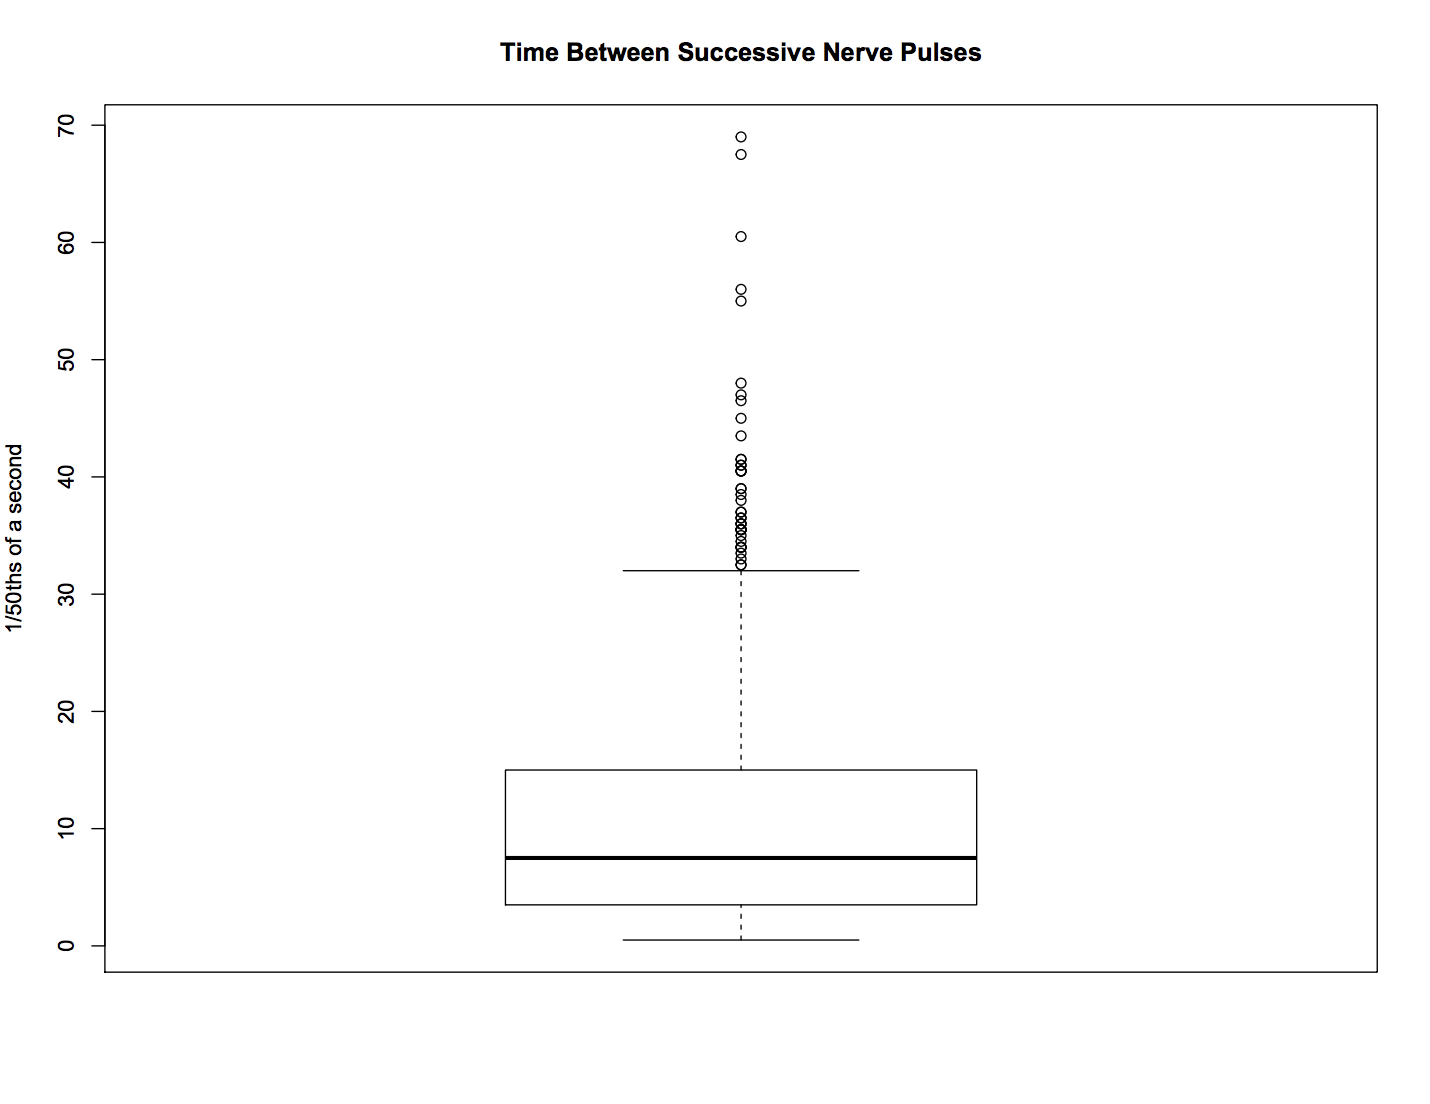
\includegraphics[width=\linewidth, height=0.27\textheight]{data.png}
		    \end{minipage}%
		    \begin{minipage}{0.5\textwidth}
		        \centering
		        \captionof{figure}{Log of Data}
		        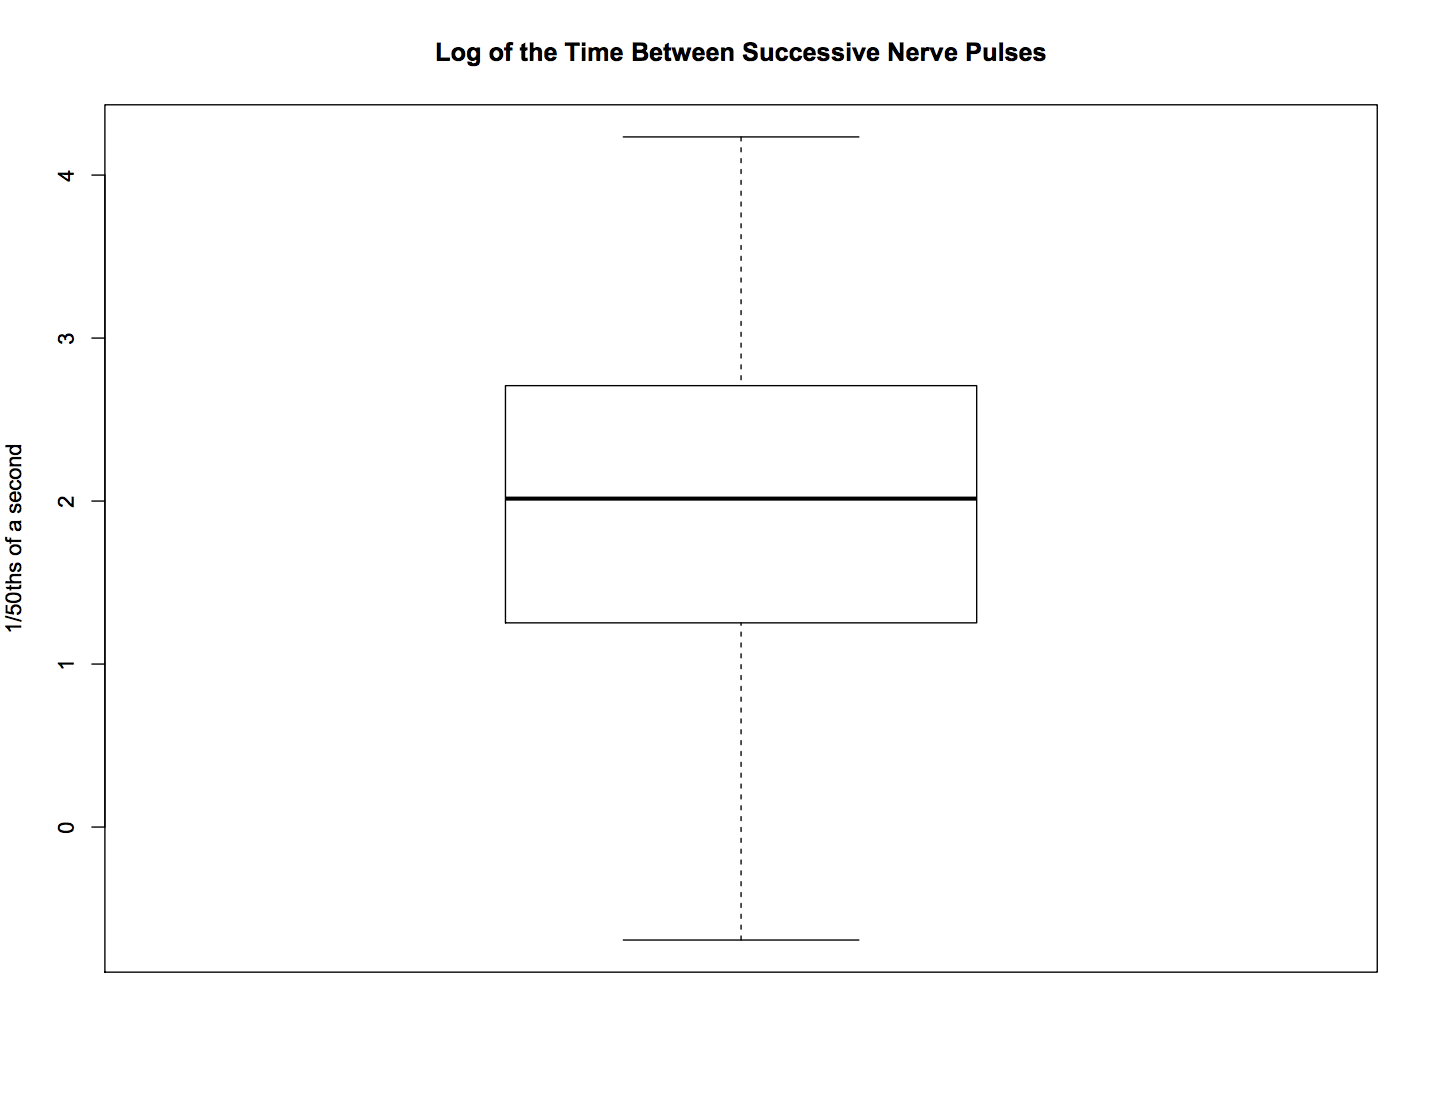
\includegraphics[width=\linewidth, height=0.27\textheight]{logdata.png}
		    \end{minipage}
		\end{figure}

		\begin{figure}[!htb]
		    \centering
		    \begin{minipage}{0.5\textwidth}
		        \centering
		        \captionof{figure}{Square Root of Data}
		        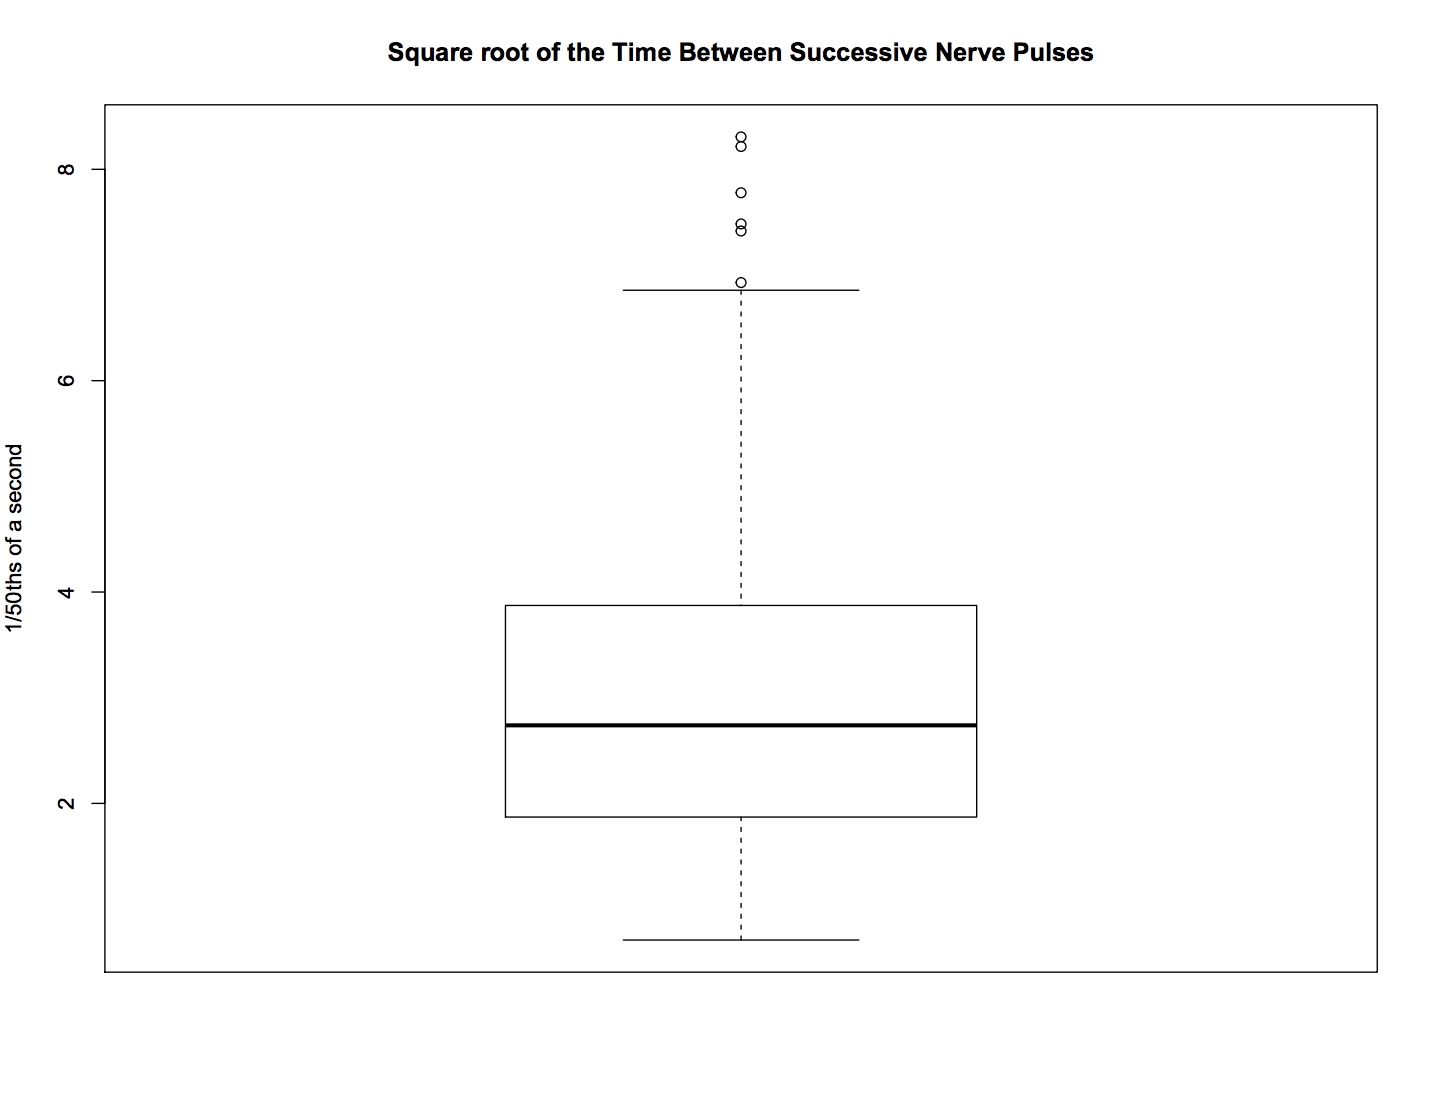
\includegraphics[width=\linewidth, height=0.27\textheight]{sqrtdata.png}
		    \end{minipage}%
		    \begin{minipage}{0.5\textwidth}
		        \centering
		        \captionof{figure}{Square of Data}
		        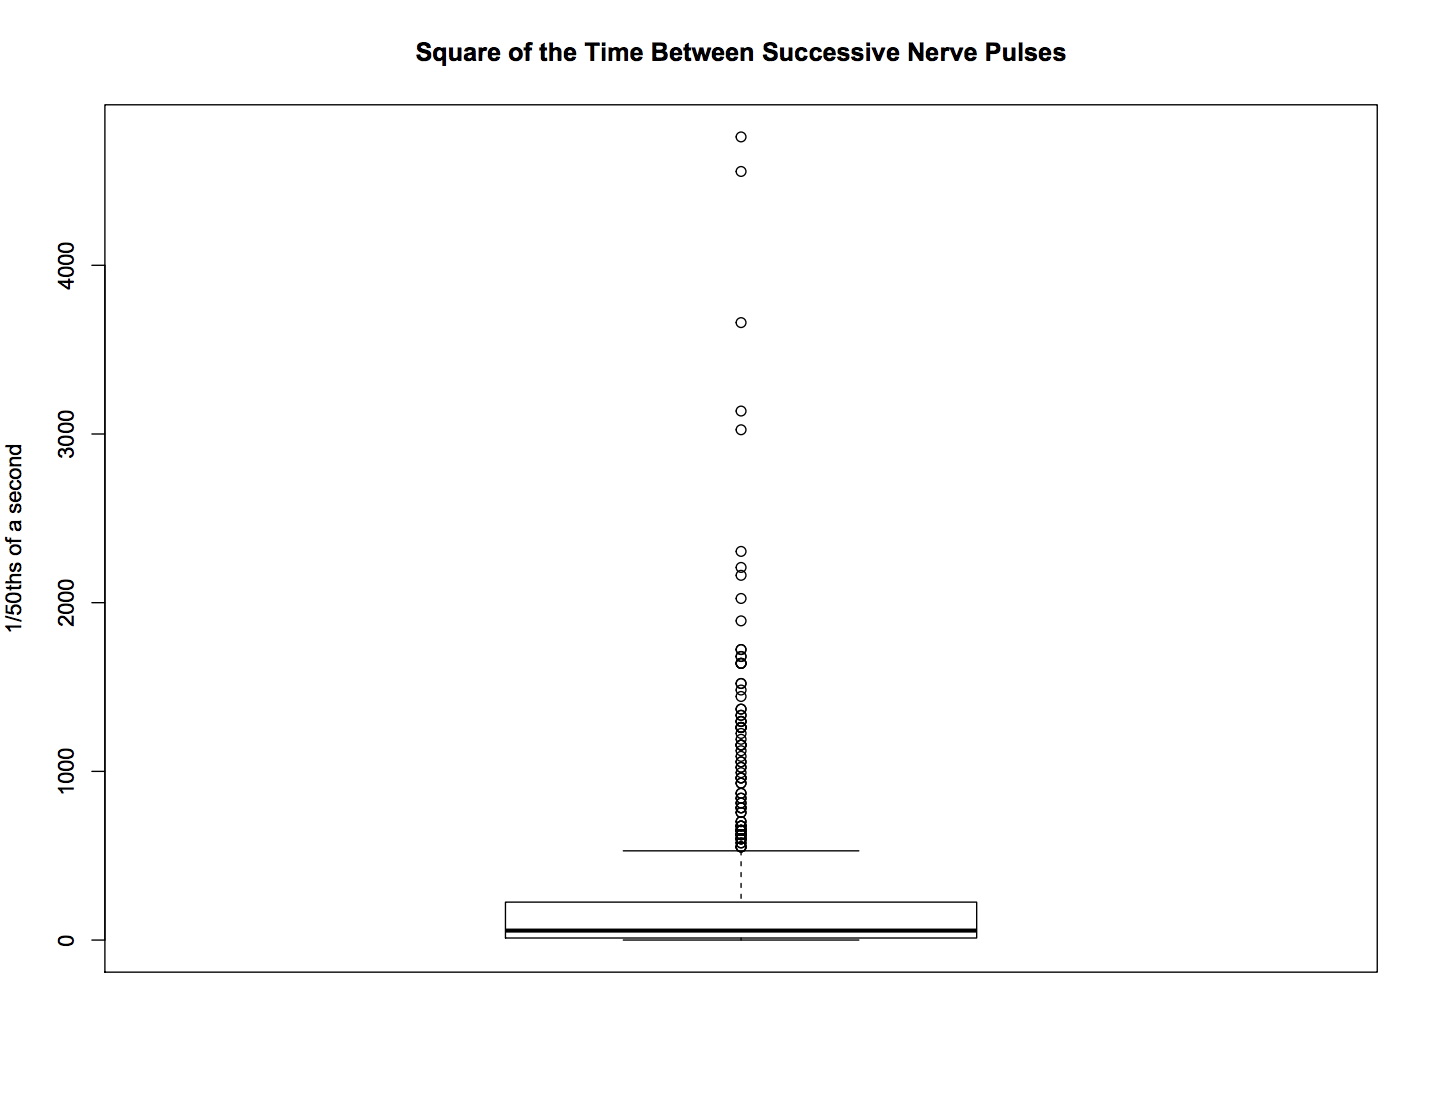
\includegraphics[width=\linewidth, height=0.27\textheight]{squaredata.png}
		    \end{minipage}
		\end{figure}

		\begin{figure}[!htb]
			\centering
		    \begin{minipage}{0.5\textwidth}
		        \centering
		        \captionof{figure}{Reciprocal of Data}
		        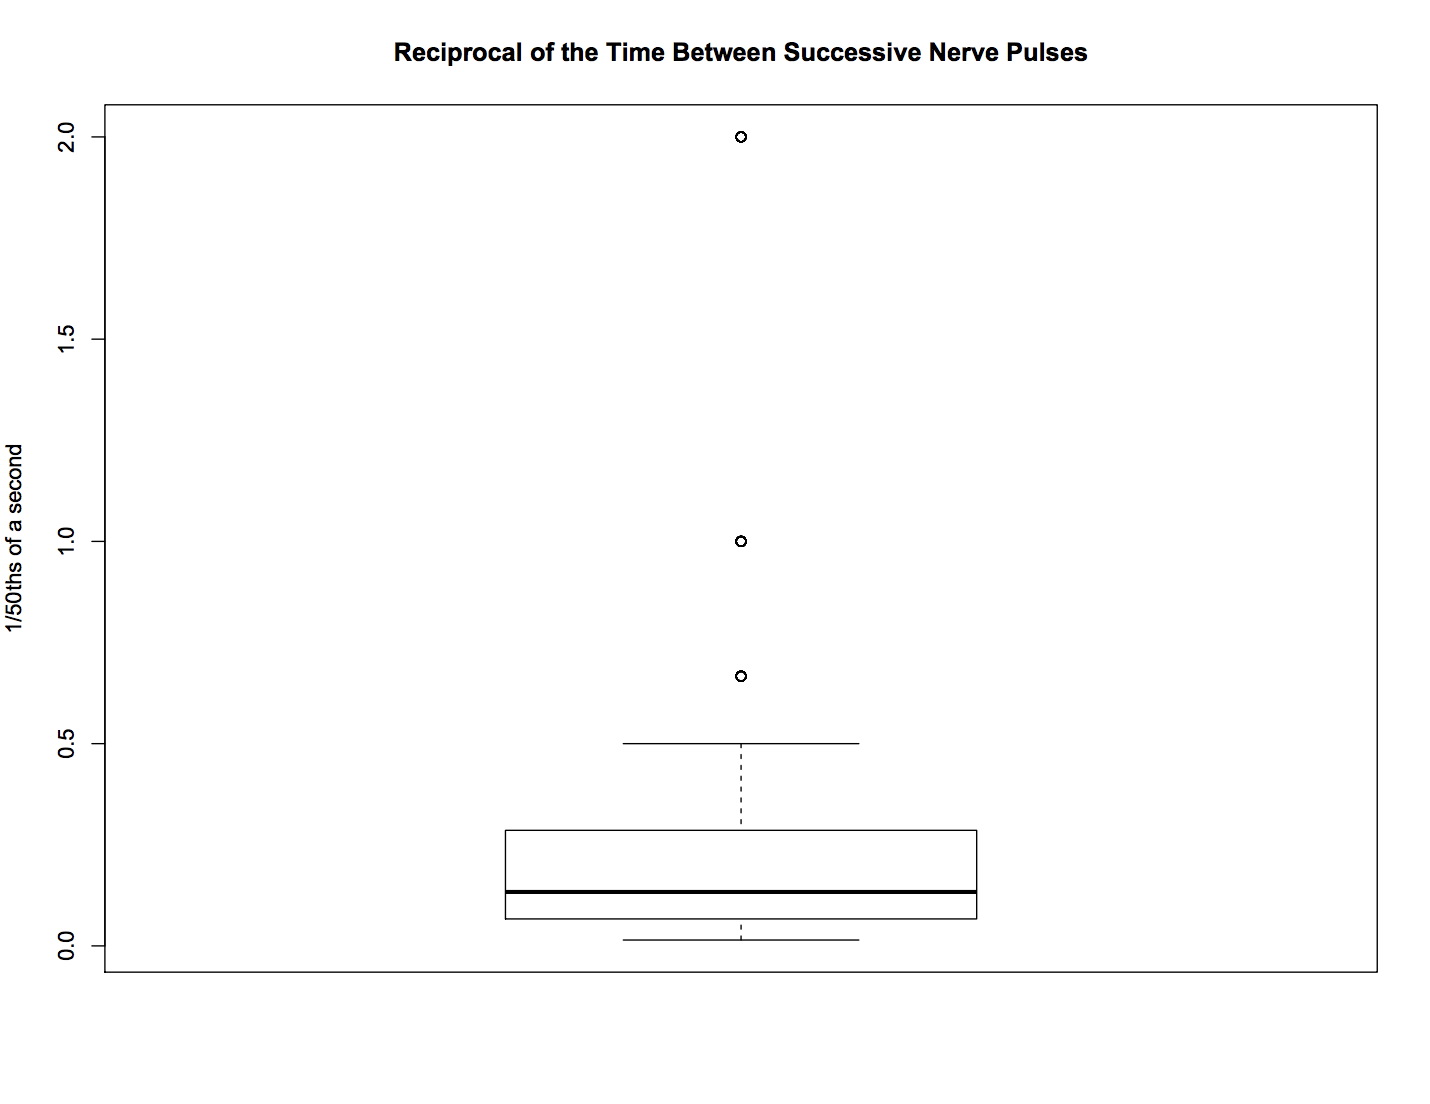
\includegraphics[width=\linewidth, height=0.27\textheight]{recipdata.png}
		    \end{minipage}%
		    \centering
		    \begin{minipage}{0.5\textwidth}
		        \centering
		        \captionof{figure}{Cube of Data}
		        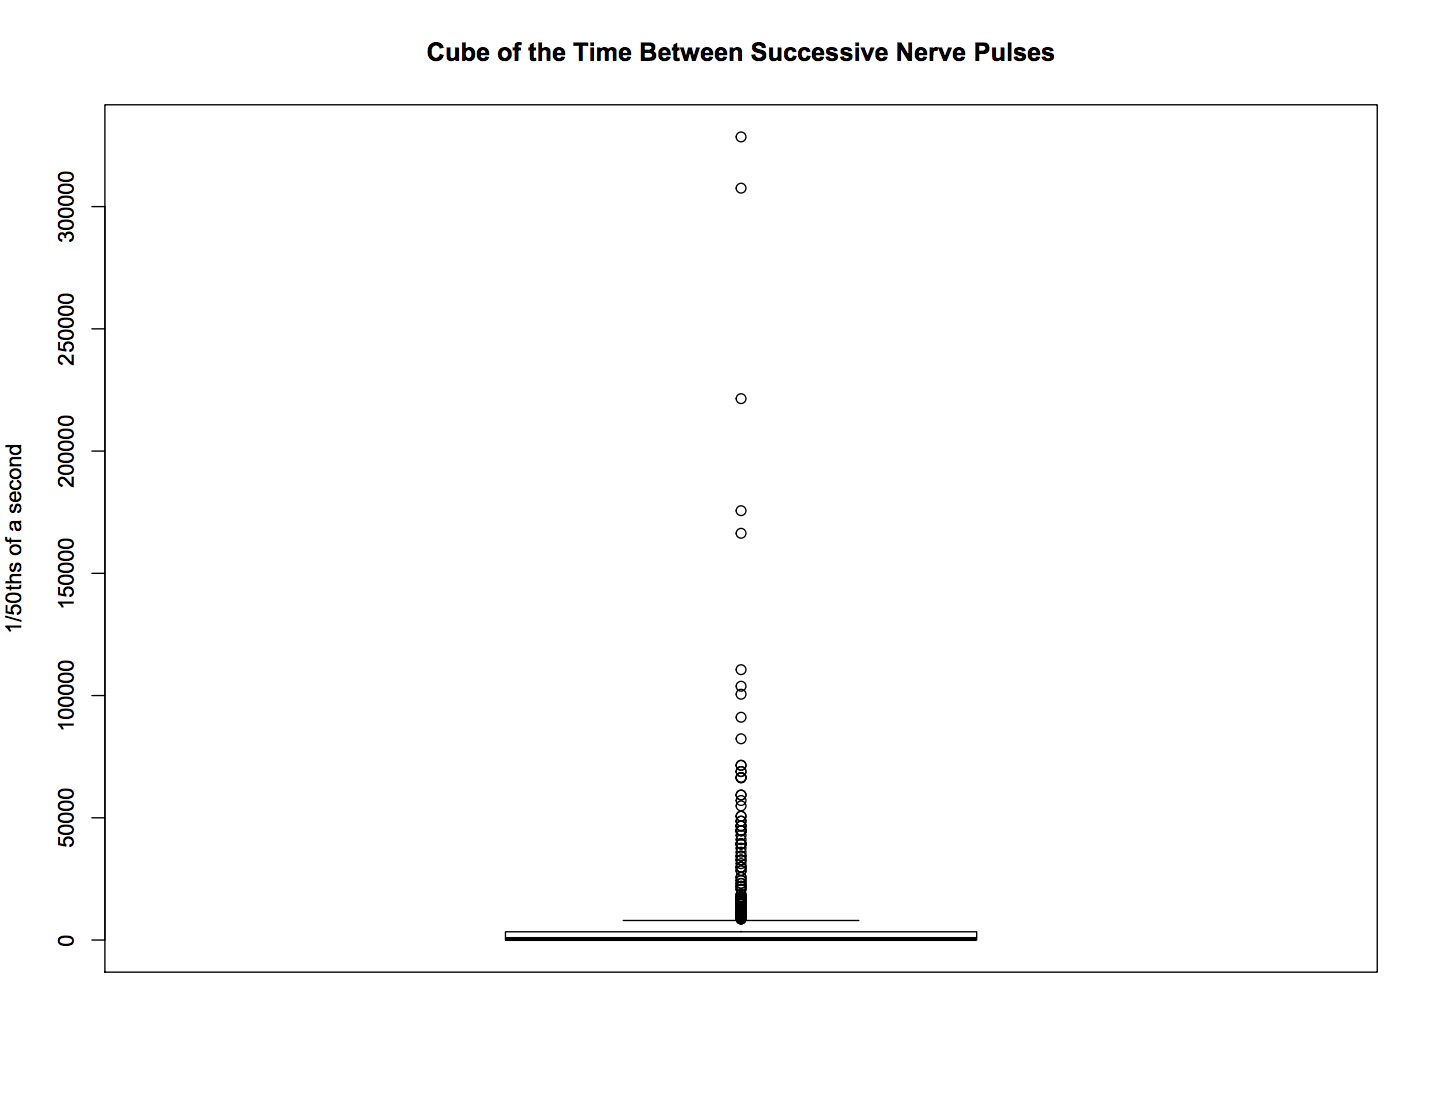
\includegraphics[width=\linewidth, height=0.27\textheight]{cubedata.png}
		    \end{minipage}
		\end{figure}

	\end{enumerate}

\end{enumerate}

\end{document}
